

\chapter{Group Theory}
In order to have a more systemetic study on topological spaces, we need to use some abstract algebra to `extract' some properties of these spaces. In this chapter, we will focus on some aspects of group theory, which is covered in any standard abstract algebra course (e.g. MAT3004). 
\section{Basic Group Theory}
When one talks about algebraic structure, we would think of addition $a + b$ and multiplication $a \cdot b$. In general, we make the following definition:
\begin{definition}
    Let $S$ be a set. A {\bf binary operation} $S$ is a map
    $$\ast: S \times S \to S.$$
    A subset $T \subseteq S$ is {\bf closed under $\ast$} if for all $a, b \in T$, $a \ast b \in T$.
\end{definition}

\begin{definition} \label{def-group}
    A group $G$ is a set along with a binary operation $\ast: G \times G \to G$ satisfying:
    \begin{itemize}
        \item $(a \ast b) \ast c = a \ast (b \ast c)$;
        \item There exists $e\in G$ such that $e \ast g = g \ast e = g$ for all $g \in G$.
        \item For all $g \in G$, there exists $g^{-1} \in G$ such that $g \ast g^{-1} = g^{-1} \ast g = e$.
    \end{itemize}
\end{definition}

\begin{example}
    \begin{enumerate}
        \item $(\mathbb{Z},+)$, $(\mathbb{Q},+)$, $(\mathbb{R},+)$, $(\mathbb{C},+)$ are groups.
        \item $(\mathbb{R}[x],+)$ is a group.
        \item (Modular arithmetic) $(\mathbb{Z}_n,+)$ is a group.
        \item As for multiplication, $(R,\cdot)$ is not a group for $R = \mathbb{Z}, \mathbb{Q}, \mathbb{R}, \mathbb{C}, \mathbb{R}[x]$ or $\mathbb{Z}_n$, since $0^{-1}$ does not exist in all cases.
        \item $\mathbb{Z} \backslash \{0\}$ is still not a group, since $3^{-1}$ does not exist. But $(\mathbb{Q}\backslash \{0\}, \cdot)$ is a group.
        \item $(GL_n(\mathbb{R}), \cdot)$ is a group under matrix multiplication.
        \item Consider the regular $n$-gon \(P_n \subseteq {\mathbb{R}}^{2}\) centered at the origin. Let \({D}_{2n}\) be the symmetries of $P_n$, for instance $r \in D_{2n}$ is the rotation of $P_n$ by $2\pi/n$ anti-clockwise about the origin, and $s \in D_{2n}$ be any reflection of $P_n$. Then obviously
        $$r^n = e, \quad s^2 = e$$
        in $D_n$. Indeed, all elements of \({D}_{2n}\) can be obtained by \({r}^{i}{s}^{j},0 \leq  i \leq  r-1,\ 0 \leq  j \leq  1\).
    \end{enumerate}
\end{example}    

\begin{definition}
    A group $(G, \ast)$ is called {\bf abelian/commutative} if
    $$a \ast b = b \ast a$$
    for all $a, b \in G$.
\end{definition}

\begin{example}
$(\mathbb{Z},+)$, $(\mathbb{Q},+)$, $(\mathbb{R},+)$, $(\mathbb{C},+)$, $(\mathbb{R}[x],+)$, $(\mathbb{Z}_n,+)$, $(\mathbb{Q}\backslash \{0\}, \cdot)$ are commutative, but $(GL_n(\mathbb{R}), \cdot)$, $(D_{2n}, \cdot)$ are not commutative.
\end{example}   


\begin{definition} Let \(G,H\) be two groups. The product group \(\left( {G \times  H, * }\right)\) is defined as
\[
G \times  H = \{ \left( {g,h}\right)  \mid  g \in  G,h \in  H\}
\]
with \(\left( {{g}_{1},{h}_{1}}\right)  * \left( {{g}_{2},{h}_{2}}\right)  = \left( {{g}_{1}{g}_{2},{h}_{1}{h}_{2}}\right)\).
\end{definition}

For example, \(\left( {\mathbb{R} \times  \mathbb{R}, + }\right)  = \{ \left( {x,y}\right)  \mid  x,y \in  \mathbb{R}\}\) coincides with the usual \({\mathbb{R}}^{2}\), where
\[
\left( {x,y}\right)  * \left( {{x}^{\prime },{y}^{\prime }}\right)  = \left( {x + {x}^{\prime },y + {y}^{\prime }}\right)
\]

Here is the analogue of `linear transformation' between two groups $G$ and $H$ in group theory:
\begin{definition} A map between two groups \(\phi  : G \rightarrow  H\) is a \emph{homomorphism} if
\[
\phi \left( {{g}_{1} * {g}_{2}}\right)  = \phi \left( {g}_{1}\right)  * \phi \left( {g}_{2}\right)
\]
In other words, a homomorphism is a map preserving multiplications of groups.
\end{definition}
Following the similar idea as in linear algebra, if \(\phi  : G \rightarrow  H\) is a homomorphism, then \(\phi \left( {e}_{G}\right)  = {e}_{H}\).

\begin{example} Let \(G = \left( {\mathbb{R},+,0}\right)\), and \(H = \left\{  {{H}_{2},*,{I}_{2}}\right\}\), with \({H}_{2}\) of the form
\[
{H}_{2} = \left\{  {\left. \left( \begin{array}{ll} 1 & x \\  0 & 1 \end{array}\right) \right| \;x \in  \mathbb{R}}\right\}
\]
Define a mapping
\[
\phi  : \;G \rightarrow  H
\]
by \(x \mapsto  \left( \begin{array}{ll} 1 & x \\  0 & 1 \end{array}\right)\). Then \(\phi\) is a homomorphism, i.e.:
\[
\phi \left( {x{ * }_{\mathbb{R}}y}\right)  = \phi \left( {x + y}\right)= \left( \begin{matrix} 1 & x + y \\  0 & 1 \end{matrix}\right)= \left( \begin{array}{ll} 1 & x \\  0 & 1 \end{array}\right) \left( \begin{array}{ll} 1 & y \\  0 & 1 \end{array}\right) = \phi \left( x\right)  *_ {{H}_{2}}\phi \left( y\right)
\]
\end{example}

\begin{definition} [Isomorphism] A homomorphism \(\phi  : G \rightarrow  H\) is an isomorphism if \(\phi\) is bijective. The isomorphism between \(G\) and \(H\) is denoted as \(G \cong  H\).
\end{definition}

\section{Free Groups}
\begin{definition}
Let \(S\) be a set (the "alphabet"). 
\begin{itemize}
\item Define \({S}^{-1} \mathrel{\text{ := }} \left\{  {s^{-1} \in  s \in  S}\right\}\) such that
\begin{itemize}
    \item \(S \cap  {S}^{-1} = \varnothing\); and
    \item the elements $(s^{-1})^{-1} \in (S^{-1})^{-1}$ satisfy \({\left( {s}^{-1}\right) }^{-1} = s\). In particular $(S^{-1})^{-1} = S$.
\end{itemize}
\item A \emph{word} in \(S\) is a finite sequence \(w = {w}_{1}\cdots {w}_{m}\), where \(m \in  {\mathbb{N}}^{ + } \cup  \{ 0\}\), and each \({w}_{i}  \in  S \cup  {S}^{-1}\). In particular, when \(m = 0\), we view \(w\) as the empty sequence, denoted as \(\varnothing\).

\item The \emph{concatenation} of two words \({x}_{1}\cdots {x}_{m}\) and \({y}_{1}\cdots {y}_{n}\) is the word \({x}_{1}\cdots {x}_{m}{y}_{1}\cdots {y}_{n}\)

\item Two words \(w,{w}^{\prime }\) are \emph{equivalent}, denoted as \(w \sim  {w}^{\prime }\), if there are words \({w}_{1},\ldots,{w}_{n}\) and \(w = {w}_{1},{w}^{\prime } = {w}_{n}\) such that $w_i$ and $w_{i+1}$ differ from each other by
\[
{w}_{i} = \cdots {y}_{1}x{x}^{-1}{y}_{2}\cdots,\quad {w}_{i + 1} = \cdots {y}_{1}{y}_{2}\cdots
\]
or
\[
{w}_{i} = \cdots {y}_{1}{y}_{2}\cdots,\quad {w}_{i + 1} = \cdots {y}_{1}x{x}^{-1}{y}_{2}\cdots
\]
for some \(x \in  S \cup  {S}^{-1}\).
\end{itemize}
\end{definition}

\begin{example} Let \(S = \{ a,b\}\) \({S}^{-1} = \left\{  {{a}^{-1}, {b}^{-1}}\right\}\) and
\[
w = {aaba}{b}^{-1}{b}^{-1}{a}^{-1}{abaab}{b}^{-1}a,
\quad {w}^{\prime } = {aaba}{b}^{-1}{b}^{-1}{a}^{-1}{abaaa}
\]
Here \(w\) and \({w}^{\prime }\) differ by \(b{b}^{-1}\). Therefore, \(w \sim  {w}^{\prime }\), and \(w\) is said to be an elementary expansion of \({w}^{\prime }\).

Moreover, for
\[
w = {aaba}{b}^{-1}{b}^{-1}{a}^{-1}{abaab}{b}^{-1}a, \quad {w}^{\prime \prime } = {aaba}{b}^{-1}{b}^{-1}{baab}{b}^{-1}a,
\]
\(w\) and \({w}^{\prime \prime }\) differ by \({a}^{-1}a\), i.e., \({a}^{-1}{\left( {a}^{-1}\right) }^{-1}\), and therefore \(w \sim  {w}^{\prime \prime }\).
\end{example}


\begin{definition} [Free Group] Let $S$ be a set. The \emph{free group} \(F\left( S\right)\) is defined to be the equivalence class of words, i.e.,
\[
\left\lbrack  w\right\rbrack   \mathrel{\text{ := }} \left\{  {{w}^{\prime }\text{ is a word in }S \mid  w \sim  {w}^{\prime }}\right\}   \in  F\left( S\right)
\]
\end{definition}

Note that \(F\left( S\right)\) is indeed a group:
\begin{itemize}
\item \(\left\lbrack  w\right\rbrack   * \left\lbrack  {w}^{\prime }\right\rbrack   = \left\lbrack  {w{w}^{\prime }}\right\rbrack\) (concatenation) check \({w}_{1} \sim  {w}_{2},{u}_{1} \sim  {u}_{2}\) implies \({w}_{1}{u}_{1} \sim\)  \({w}_{2}{u}_{2}\)

\item Identity element: \(e = \left\lbrack  \varnothing \right\rbrack\)

\item Inverse element: \({\left\lbrack  {x}_{1}\cdots {x}_{n}\right\rbrack  }^{-1} = \left\lbrack  {{x}_{n}^{-1}\cdots {x}_{1}^{-1}}\right\rbrack\)
\end{itemize}

\begin{example} Let \(S = \{ a\}\) and \({S}^{-1} = \left\{  {a}^{-1}\right\}\). Any word \(w\) has the form
\[
w = a\cdots a{a}^{-1}\cdots {a}^{-1}a\cdots a{a}^{-1}\cdots {a}^{-1}\cdots
\]
In shorthand, we denote \(w\) as \(w = \cdots {a}^{p}{\left( {a}^{-1}\right) }^{q}{a}^{r}{\left( {a}^{-1}\right) }^{s}\cdots\), and
\[
\left\lbrack  w\right\rbrack   = \left\lbrack  {\cdots {a}^{p}{\left( {a}^{-1}\right) }^{q}{a}^{r}{\left( {a}^{-1}\right) }^{s}\cdots }\right\rbrack   = \left\lbrack  {\cdots {a}^{p - 1}{\left( {a}^{-1}\right) }^{q - 1}{a}^{r}{\left( {a}^{-1}\right) }^{s}\cdots }\right\rbrack
= \left\lbrack  {\cdots {a}^{p - 1}{\left( {a}^{-1}\right) }^{q - 2}{a}^{r - 1}{\left( {a}^{-1}\right) }^{s}\cdots }\right\rbrack
\]
For instance, we can always eliminate the adjacent terms \(a\) and \({a}^{-1}\) up to equivalence class. Therefore, 
\[F\left( S\right)  = \left\{  {\cdots,\left\lbrack  {a}^{-2}\right\rbrack ,\left\lbrack  {a}^{-1}\right\rbrack ,\left\lbrack  \varnothing \right\rbrack ,\left\lbrack  a\right\rbrack ,\left\lbrack  {a}^{2}\right\rbrack ,\cdots }\right\}.\]
It is clear that \(F\left( S\right)  \cong  \mathbb{Z}\), where the isomorphism \(\phi  : \mathbb{Z} \rightarrow  F\left( S\right)\) is \(\phi \left( n\right)  = \left\lbrack  {a}^{n}\right\rbrack\).
\end{example}

\begin{example} Let \(S = \{ a,b\}\) and \({S}^{-1} = \left\{  {{a}^{-1},{b}^{-1}}\right\}\). In this case, \(\left\lbrack  {ab}\right\rbrack   \neq  \left\lbrack  {ba}\right\rbrack\), and \(\left\lbrack  {a{b}^{-1}{a}^{2}{b}^{2}{a}^{-2}b}\right\rbrack\) cannot be reduced further.

Since \(F(S)\) is not an abelian group, we imply \(F\left( S\right) \ncong \mathbb{Z} \times  \mathbb{Z}\).
\end{example}


\begin{definition} [Group With Relations] Let \(S\) be a set. A group with relations is written as
\[
G = \langle S \mid  R\left( S\right) \rangle
\]
where \(R\left( S\right)\) consists of elements in \(F\left( S\right)\), and every element in \(G\) can be written as the form \(\left\lbrack  w\right\rbrack\) for some  \(w  \in  F\left( S\right)\). We insist that \(\left\lbrack  w\right\rbrack   = \left\lbrack  {w}^{\prime }\right\rbrack\) in \(G\) iff 
\begin{itemize}
\item \(w\) and \({w}^{\prime }\) differ by some \(x{x}^{-1},x \in  S \cup  {S}^{-1}\), or
\item \(w\) and \({w}^{\prime }\) differ by some element \(z \in  R\left( S\right)\), or its inverse.
\end{itemize}
(One can easily check the above two conditions defines an equivalence relationship $\sim$ on $F(S)$, and hence $[w] \in G := F(S)/ \sim$ can be seen as the equivalence class with representative $w$. 
\end{definition}

\begin{example} Let 
\[G = \left\langle  {a,b \mid  {a}^{2},{b}^{2},{aba}{b}^{-1}{a}^{-1}{b}^{-1}}\right\rangle.\] 
We want to enumerate all possible elements in \(G\). To do so, observe that
\[
\left\lbrack  {b}^{-1}\right\rbrack   = \left\lbrack  {{b}^{-1}{b}^{2}}\right\rbrack   = \left\lbrack  b\right\rbrack ,\quad \left\lbrack  {a}^{-1}\right\rbrack   = \left\lbrack  a\right\rbrack,
\quad
\left\lbrack  {bab}\right\rbrack   = \left\lbrack  {{aba}{b}^{-1}{a}^{-1}{b}^{-1}{bab}}\right\rbrack   = \left\lbrack  {{aba}{b}^{-1}b}\right\rbrack   = \left\lbrack  {aba}\right\rbrack
\]
As a result,
\begin{itemize}
\item \(\left\lbrack  {a}^{-n}\right\rbrack   = \left\lbrack  {a}^{n}\right\rbrack\) and \(\left\lbrack  {b}^{-n}\right\rbrack   = \left\lbrack  {b}^{n}\right\rbrack\)
\item \(\left\lbrack  {a}^{{2n} + 1}\right\rbrack   = \left\lbrack  a\right\rbrack ,\left\lbrack  {b}^{{2n} + 1}\right\rbrack   = \left\lbrack  b\right\rbrack ,\left\lbrack  {a}^{2n}\right\rbrack   = \left\lbrack  \varnothing \right\rbrack ,\left\lbrack  {b}^{2n}\right\rbrack   = \left\lbrack  \varnothing \right\rbrack\)
\item All elements of \(G\) are of the form \(\left\lbrack  {\cdots {abababab}\cdots }\right\rbrack\).
\end{itemize}
Moreover, since each $aba$ can be changed into \({bab}\), the elements in \(G\) are
\[
\left\lbrack  \varnothing \right\rbrack ,\left\lbrack  a\right\rbrack ,\left\lbrack  b\right\rbrack ,\left\lbrack  {ab}\right\rbrack ,\left\lbrack  {ba}\right\rbrack ,\left\lbrack  {aba}\right\rbrack
\]
In fact, \(G \cong D_6 (\cong {S}_{3})\), where $S_3 := \{ \mu: \{1,2,3\} \to \{1,2,3\}\ |\ \mu\ \text{is bijective}\}$ is the symmetric (or permutation) group of $3$ elements. There are $6 = 3!$ elements of $S_3$:
\begin{center}
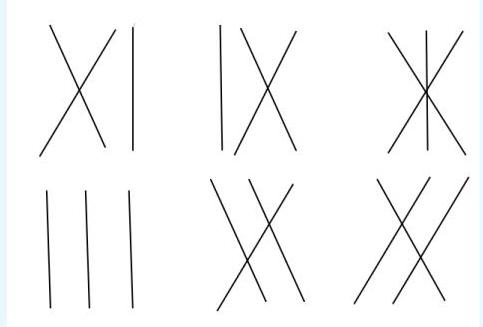
\includegraphics[width=0.5\textwidth]{images/Ch6_symmetric_group.jpg}
\end{center}
for instance, $\times \mid$ is the bijection 
\begin{center}
$1 \mapsto 2$, $2 \mapsto 1$, $3 \mapsto 1$
\end{center}
and $\mid \times$ is the bijection
\begin{center}
$1 \mapsto 1$, $2 \mapsto 3$, $3 \mapsto 2$.
\end{center}
Then the isomorphism \(\phi  : {S}_{3} \rightarrow  G
\) is given by:
where $\phi(\times \mid) = a$, $\phi(\mid  \times) =  b$.
\end{example}

\begin{example}
\begin{enumerate}
    \item The dihedral group $D_{2n}$ is isomorphic to (or one can simply take this as a definition):
\[
D_{2n} :=\left\langle  {a,b \mid  {a}^{n} = e,{b}^{2} = e,{bab} = {a}^{-1}}\right\rangle
\]
\item Consider \({G} =  < a,b \mid  {ab} = {ba} >\). Then any element of $G$ can be expressed as \([\cdots {a}^{s}{b}^{t}{a}^{u}{b}^{v}\cdots]\). Using the relations \({ab} = {ba}\) and $b{a}^{-1} = {a}^{-1}b$, we can always push all powers of \(a\) to the left.

Therefore, all elements in \({G}\) are of the form \([{a}^{p}{b}^{q}],\ p,q \in  \mathbb{Z}\), and we have the relation
\[
\left[ {{a}^{{p}_{1}}{b}^{{q}_{1}}}\right] \left[ {{a}^{{p}_{2}}{b}^{{q}_{2}}}\right] = [{a}^{{p}_{1} + {p}_{2}}{b}^{{q}_{1} + {q}_{2}}].
\]
Therefore, \({G} \cong  \mathbb{Z} \times  \mathbb{Z}\), where the isomorphism is given by:
\[
\phi  : \;\mathbb{Z} \times  \mathbb{Z} \rightarrow  {G}_{2}
\]
with \(\left( {p,q}\right)  \mapsto  [{a}^{p}{b}^{q}].\)

\item Let \[
H = \left\langle  {a \mid  {a}^{5}}\right\rangle   = \left\{  {1,a,{a}^{2},\ldots,{a}^{4}}\right\}
\]
It’s clear that \(H \cong  \mathbb{Z}/5\mathbb{Z}\), where the isomorphism is given by:
\[
\phi  : \;\mathbb{Z}/5\mathbb{Z} \rightarrow  H
\]
with \(m + 5\mathbb{Z} \mapsto  [{a}^{m}].\)
\end{enumerate}
\end{example}

\section{Cayley Graph for finitely presented groups}
Graphs have strong connection with groups. Here we introduce a way of building graphs using groups, and the graphs are known as Cayley graphs. They describe many properties of the group in a topological way.

\begin{definition} [Oriented Graph] An oriented graph \(T\) is specified by

1. A countable or finite set \(V\), known as vertices

2. A countable or finite set \(E\), known as edges

3. A function \(\delta  : E \rightarrow  V \times  V\) given by
\[
\delta \left( e\right)  = \left( {\ell \left( e\right),\tau \left( e\right) }\right)
\]
where \(\ell \left( e\right)\) denotes the initial vertex and \(\tau \left( e\right)\) denotes the terminal vertex.
\end{definition}

For example, let
\begin{itemize}
\item \(V = \{ a,b,c\}\)
\item \(E = \left\{  {{e}_{1},{e}_{2},{e}_{3},{e}_{4}}\right\}\)
\item \(\delta \left( {e}_{1}\right)  = \left( {a,a}\right),\delta \left( {e}_{2}\right)  = \left( {b,c}\right),\delta \left( {e}_{3}\right)  = \left( {a,c}\right),\delta \left( {e}_{4}\right)  = \left( {b,c}\right)\)
\end{itemize}
Then its oriented graph looks like:
\begin{center}
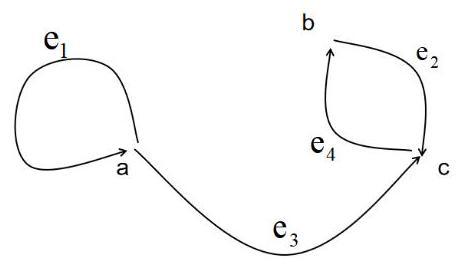
\includegraphics[width=0.3\textwidth]{images/Ch6_oriented_graph.jpg}
\end{center}

\begin{definition} [Cayley graph] Let \(G = \langle S \mid  R\left( S\right) \rangle\) with \(\left| S\right|  < \infty\). The Cayley graph associated to \(G\) is an oriented graph with

1. The vertex set \(G\)

2. The edge set \(E \mathrel{\text{ := }} G \times  S\)

3. The function \(\ell  : E \rightarrow  V \times  V\) is given by:
\[\ell  : \;G \times  S \rightarrow  G \times  G\]
with \(\left( {g,s}\right)  \mapsto  \left( {g,g \cdot  s}\right)\). In particular, we link two elements in \(G\) if they differ by a generator multiplied on the right.
\end{definition}

\begin{example}
\begin{enumerate}
    \item The Cayley graph for \(G = \langle a\rangle \left( { \cong  \mathbb{Z}}\right)\) is shown below:
\begin{center}
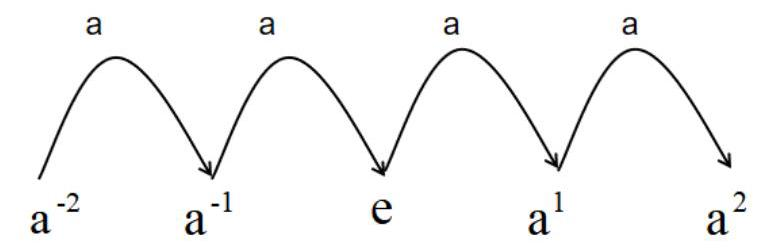
\includegraphics[width=0.5\textwidth]{images/Ch6_graph_Z.jpg}
\end{center}


\item The Cayley graph for \(G = \left\langle  {a \mid  {a}^{3}}\right\rangle\) is:

\begin{center}
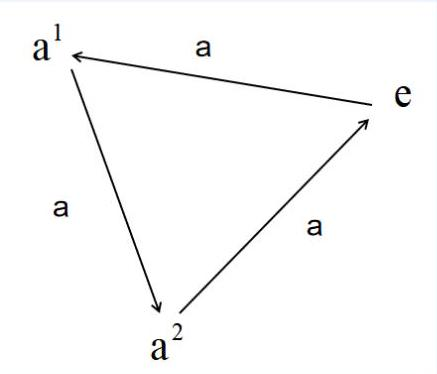
\includegraphics[width=0.3\textwidth]{images/Ch6_graph_Z3.jpg}
\end{center}

\item The Cayley graph for \(G = \left\langle  {a,b \mid  {a}^{2},{b}^{2},{aba} = {bab}}\right\rangle\) is:

\begin{center}
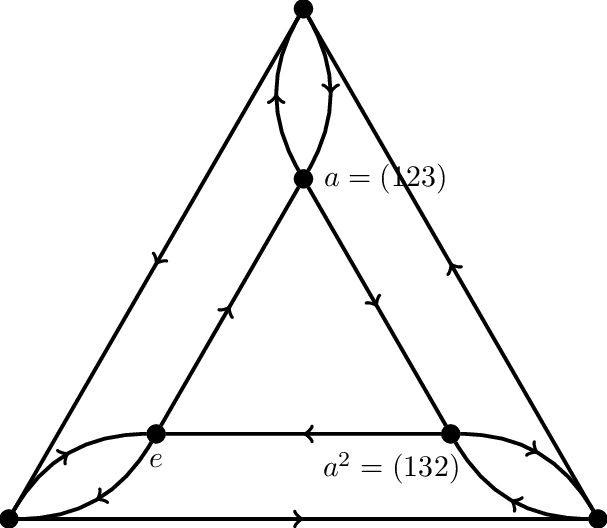
\includegraphics[width=0.35\textwidth]{images/Ch6_graph_S3.png}
\end{center}

\item The Cayley graph for \(G = \langle a,b \mid  {ab} = {ba}\rangle\) is:

\begin{center}
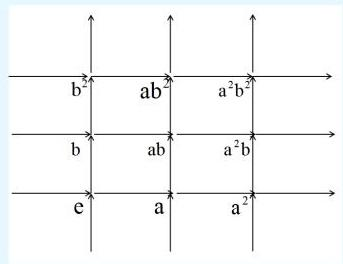
\includegraphics[width=0.4\textwidth]{images/Ch6_graph_ZZ.jpg}
\end{center}


\item The Cayley graph for \(G = \langle a,b\rangle\) is:

\begin{center}
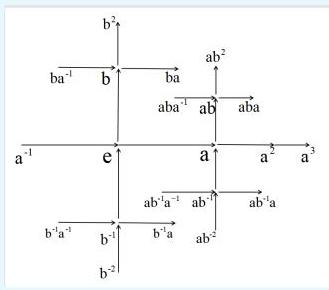
\includegraphics[width=0.5\textwidth]{images/Ch6_graph_F2.jpg}
\end{center}
\end{enumerate}
\end{example}